\subsection{Applikation}

\subsubsection{Funktion}

Die Applikation ist ein eigenständiges Programm.
Dieses kommuniziert mit dem Treiber über \gls{ioctl}.
Das Programm ist in \textit{Python} implementiert.

Das Programm ließt periodisch einen Temperatur-Messwert $\texttt{M}_C[n]$ in \si{\celsius} aus und bildet diesen zu einem \gls{pwm}-Duty Cycle $\texttt{D}[n]$ nach dem Prinzip von \autoref{eq:app}
\begin{equation}
    f \left( \texttt{M}_C \left[n\right] \right) \rightarrow \texttt{D}\left[n\right]
    \label{eq:app}
\end{equation}

Grundsätzlich kann die Übertragungsfunktion $f$ beliebig implementiert werden.
Diese kann sogar von historischen Messdaten $\texttt{M}_C[n-m]$ abhängig sein.
Unsere implementation realisiert zur Demonstration einen einfachen, kontextfreien, \gls{lut}.
Dieser beinhält einzelne Eingabe/Ausgabe Wert Datenpaare aus einer \gls{csv} Datei und bestimmt den momentanen Ausgang anhand von linearer Interpolation am Eingangswert.
Die resultierende Übertragungsfunktion ist eine stückweis lineare Funktion.
Ein Beispiel dafür ist in \autoref{fig:pcl} dargestellt.

\begin{figure}
    \centering
    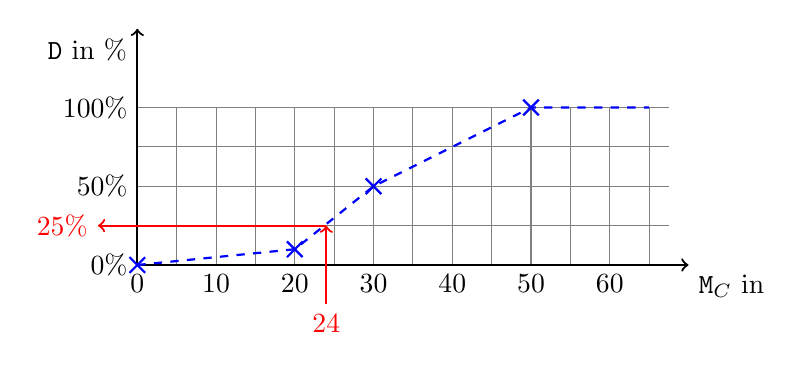
\begin{tikzpicture}
        \draw[step=0.5,gray,thin] (0,0) grid (6.75,2);
        \draw[thick, ->] (0,0) -- ++(7,0) node[below right] {$\texttt{M}_C$ in \si{\celsius}};
        \draw[thick, ->] (0,0) -- (0,3) node[below left] {$\texttt{D}$ in \%};
        \draw (0,0) node[left]  {$0\%$};
        \draw (0,1) node[left]  {$50\%$};
        \draw (0,2) node[left]  {$100\%$};
        \draw (0,0) node[below] {$0\si{\degree}$};
        \draw (1,0) node[below] {$10\si{\degree}$};
        \draw (2,0) node[below] {$20\si{\degree}$};
        \draw (3,0) node[below] {$30\si{\degree}$};
        \draw (4,0) node[below] {$40\si{\degree}$};
        \draw (5,0) node[below] {$50\si{\degree}$};
        \draw (6,0) node[below] {$60\si{\degree}$};
        \draw[thick, blue] plot[mark=x, mark size=4pt, only marks] coordinates {(0,0) (2,0.2) (3, 1) (5,2)};
        \draw[thick, blue, dashed] plot[] coordinates {(0,0) (2,0.2) (3, 1) (5,2) (6.5,2)};
        \draw[thick, red, ->] (2.4, 0.5) -- (-0.5,0.5) node[left] {\textcolor{red}{$25\%$}};
        \draw[thick, red, ->] (2.4, -0.5) node[below] {\textcolor{red}{$24\si{\celsius}$}} -- (2.4,0.5);
    \end{tikzpicture}
    \caption[Applikations \acrshort{lut} Beispiel]{Applikations \acrshort{lut} Beispiel. Die \textcolor{blue}{blauen Punkte} bilden den \gls{lut}. Die \textcolor{blue}{blaue Linie} zeigt die lineare interpolation. Die \textcolor{red}{rote Intersektion} zeigt einen Beispielswert und dessen dazugehöriges Interpolationsresultat an.}
    \label{fig:pcl}
\end{figure}

\subsubsection{\acrshort{ipc} über \acrshort{ioctl}}

\subsubsection{Installation und Ausführung}

Zur Ausführung wird eine globale Instanz von \textit{Python} Version \texttt{3.x.x} benötigt.
Es werden externe Abhängigkeiten benötigt.
Es wird empfohlen diese in ein lokales \texttt{virtual enviornment} zu installieren um den globalen scope nicht zu vermüllen.
Der empfohlene Prozess zur Ausführung:
\begin{lstlisting}
cd app
python3 -m venv venv
source ./venv/bin/activate
pip install -r requirements.txt
chmod +x ./app.py #optional
./app.py
\end{lstlisting}
